\documentclass{life-fr}

\begin{document}

\title{La Vie est un Jeu}
\subtitle{Réalisation de l'Étude Détaillée}
\member{Lepage Barbara}{db0company@gmail.com}
\member{Caradec Guillaume}{guillaume.caradec@gmail.com }
\member{El-Outmani Youssef}{youssef.eloutmani@gmail.com}
\member{Glorieux François}{fra.glorieux@gmail.com}
\member{Klarman Nicolas}{nickoas@gmail.com}
\member{Lassagne David}{david.lassagne@gmail.com}
\member{Le-Cor Wilfried}{wilfried.lecor@gmail.com}
\member{Lenormand Frank}{lenormf@gmail.com}
\member{Louvigny Guillaume}{guillaume@louvigny.fr}

\summary
{
  L'étude détaillée est un des rendus de l'EIP. Le RED a pour objectif la description complète sur le plan
  fonctionnel du projet et aboutit à la rédaction d'un rapport qui sera à rendre. À la suite de ce rapport, le
  projet aura une version de base des fonctionnalités.
}

\maketitle

\chapter*{Table des révisions}
%%\textbf{Table des révisions}\\

\revision{1.0}{Barbara Lepage}{Plan et Rappel de l'EIP}{25/03/2012}
\revision{1.1}{Guillaume Caradec}{But et destinataires du projet}{25/03/2012}
\revision{1.2}{David Lassagne}{L'inscription, les 5 premières minutes}{25/03/2012}
\revision{1.3}{Guillaume Louvigny}{Vue d'ensemble de la page d'accueil}{25/03/2012}
\revision{1.4}{Youssef El-Outmani}{Onglet Achievements}{25/03/2012}
\revision{1.5}{François Glorieux}{L'onglet Flux}{25/03/2012}
\revision{1.6}{David Lassagne}{Smartphone}{25/03/2012}
\revision{1.7}{Youssef El-Outmani}{Ressources}{25/03/2012}
\listofrevisions

\newpage

\tableofcontents

\chapter{Rappel de l'EIP}
\section{Qu'est-ce qu'un EIP et Epitech}
Epitech est une école formant des experts en informatique. Sa pédagogie par projet implique directement les étudiants dans leur apprentissage et les rend plus à même de réagir et s'adapter aisément, par exemple aux évolutions technologiques qui auront lieu au cours de leur carrière.\\

Un Epitech Innovative Project ou EIP est l'élément clé du cursus Epitech. Il s'agit d'un projet de fin d'études regroupant un minimum de six étudiants autour d'un but commun. Ce projet est conduit sur une durée de trois ans, beaucoup plus importante que celles des projets réalisés lors des trois premières années d'études. De plus, l'EIP amène les étudiants à se confronter au monde de l'entreprise.

\section{Sujet de ``La vie est un Jeu''}
Dans le cadre de notre EIP, nous avons décidé de réaliser un réseau social à but ludique basé sur les « bucket lists ». Une bucket list est « une liste de chose à faire avant de mourir » : elle définit toutes les choses que son auteur désire faire de son existence, une sorte de mémo pour ne pas gâcher sa vie. Notre projet permettra à nos visiteurs de construire leurs propres listes, faire valider leurs exploits, tout en le partageant avec leurs réseaux sociaux. Ainsi, chaque action réalisée par un utilisateur (ajout d'une activité, succès ou échec) sera un fil de discussion dans lequel le visiteur et son réseau pourra discuter et partager différents types de médias (photos, vidéos, etc). L'activité d'un utilisateur sera validée par son propre réseau et apparaîtra sous forme de “succès”, comme dans un jeu vidéo. Le site s'étendra par la suite en proposant d'autres caractéristiques propres aux jeux vidéos.

\chapter{But et destinataires du projet}

Le projet a pour but de créer une communauté d'utilisateurs autour d'un système d'achievement, directement lié à la vie quotidienne, aux passions ou à la vie professionnelle.\\

Les utilisateurs ciblés sont très nombreux. En théorie, toute personne ayant un centre d'interêt ou une passion est une cible.\\

À plus long terme, des partenariats commerciaux permettront de cibler des marques et des lieux.\\

Le site sera multilingue donc ouvert à l'internationalisation.

\chapter{Description fonctionnelle utilisateur}

\section{Le Site Web}

\subsection{Vue d'ensemble de la page d'accueil avant le login}

L'utilisateur verra en premier lieu un diaporama mettant en avant les dernières catégories majeures d'achievements, les achievements les plus populaires et les diverses fonctions du site. Ce diaporama aura pour but d'inciter à l'inscription de l'utilisateur.\\

La page d'accueil permettra également à l'utilisateur de s'inscrire au site. Cette inscription est détaillée plus loin.\\

La dernière fonctionnalité principale de cette page d'accueil est la connexion de l'utilisateur au site.\\

L'entrée du site pourrait éventuellement permettre de rechercher les achievements/catégories du site.

\subsection{L'inscription, les 5 premières minutes !}

L'objectif de cette étape serait clairement d'éviter toute la lourdeur que représente la récolte d'information que le site a besoin d'effectuer auprès du futur utilisateur (présenter un formulaire compact et sauvage à des chances de rebuter celui-ci et éventuellement de le faire renoncer à son inscription).\\

Nous avons donc pensés à un système en mode pas à pas, qui, tout en faisant découvrir notre outil et son univers à l'internaute, lui ferait de subtiles demandes d'informations de façon régulière, et ce afin d'alléger cette étape essentielle qui nous permettra de catégoriser le nouvel inscrit et de lui proposer du contenu en fonction de ces informations qui auront été récoltées.\\

En plus de combiner le rôle de “guide” pour la découverte du site, et de “sondeur” pour la récolte d'informations, cette méthode a pour avantage de pousser l'utilisateur à aller au bout de la présentation, et donc de l'inscription, au fur et à mesure de son avancée (Effet psychologique, il veut finir ce qu'il a commencé, puisqu'il a déjà commencé à contribuer, autant aller jusqu'au bout). La présentation allant, l'intérêt croissant, les chances d'une inscription augmentent à l'arrivée.\\
\\

Dans l'état actuel on imagine comme première approche une question simple qui amène à faire une simple action en mode ``vous êtes à un clic de rentrer dans notre univers'' avec, par exemple, le choix du genre : Homme, Femme, Non précisé.

\begin{figure}[H]
  \begin{center}
    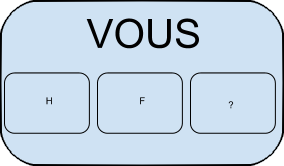
\includegraphics[width=10cm]{img/vous.png}
  \end{center}
\end{figure}

\subsection{La page d'accueil utilisateur une fois logué}

La page d'accueil de l'utilisateur habitué au site présente son flux d'informations, à l'image des flux habituels de sites communautaires tels que Facebook ou Google+. \\

Le menu doit être discret. L'utilisateur doit tout de suite voir les 4 onglets principaux :

\begin{itemize}
  \item Le flux (page d'accueil par défaut)
  \item Les objectifs de l'utilisateurs (les achievements auquel il est inscrit)
  \item Les achievements
  \item Les “amis” de l'utilisateur (importé des réseaux sociaux ou ajoutable dans le cadre du site)
\end{itemize}

Une barre de “breaking news” en permanence en haut du site donnera à l'utilisateur en une ligne les derniers achievements de ses amis ainsi que les news du site.

\begin{figure}[H]
  \begin{center}
    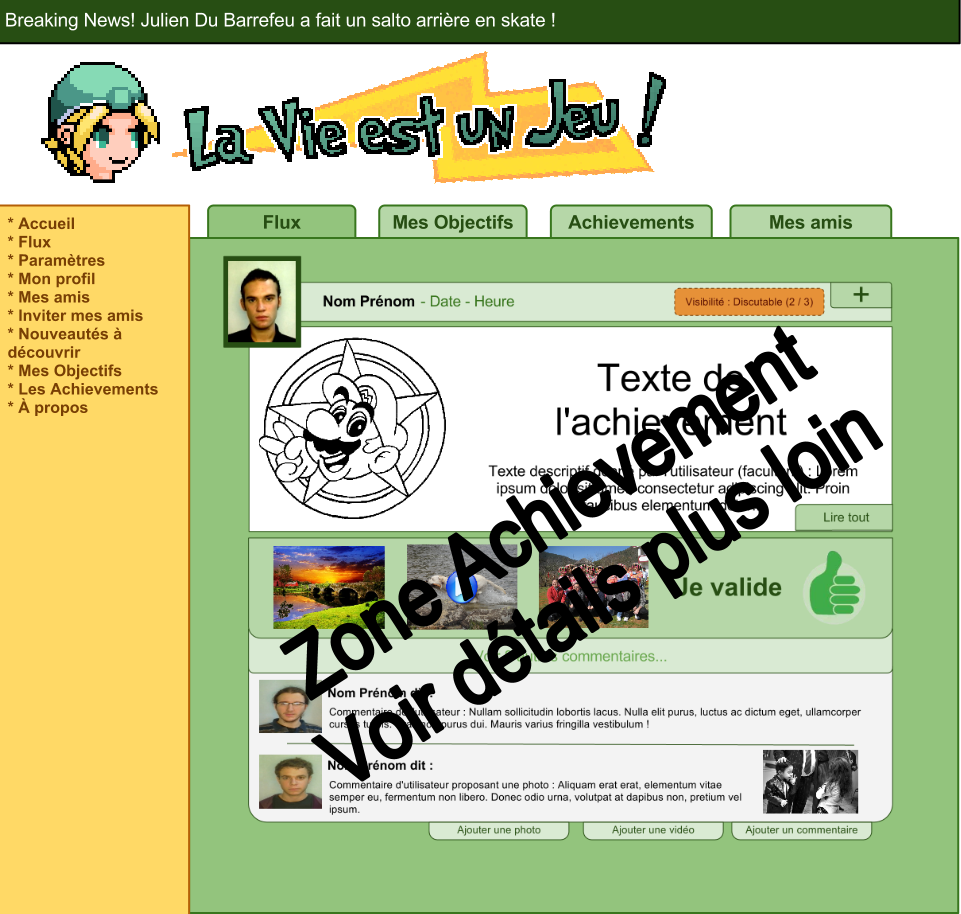
\includegraphics[width=15cm]{img/accueil.png}
  \end{center}
\end{figure}


\subsection{Onglet Flux (Feed)}

L'onglet Flux sera situé au milieu de la page principale et aura pour fonction d'afficher les derniers achievements à valider par le cercle d'amis.\\

Ce flux contiendra toutes les actions des contacts :

\begin{itemize}
  \item Les achievements à valider (voir détail ci-dessous)
  \item Les objectifs qu'ils se sont fixés
  \item Les nouveaux contacts
  \item Des nouveautés du site (informations ou nouveaux achievements)
\end{itemize}

\subsection{Détails d'un achievement}

Chaque achievement disposera d'une fonction Like qui permettra aux utilisateurs d'indiquer qu'ils aiment la publication en question, ainsi que d'un module d'envoi de preuves d'achievements servant à la validation. Le support de validation pourra être au format texte, photo ou vidéo. La photo de l'utilisateur apparaîtra ainsi que la description de l'achievement, en regard de celle-ci. Il sera également possible de poster des commentaires en-dessous des preuves de validation. Un onglet « Plus » permettra de dérouler chaque achievement afin d'obtenir plus d'informations.\\

\begin{figure}[H]
  \begin{center}
    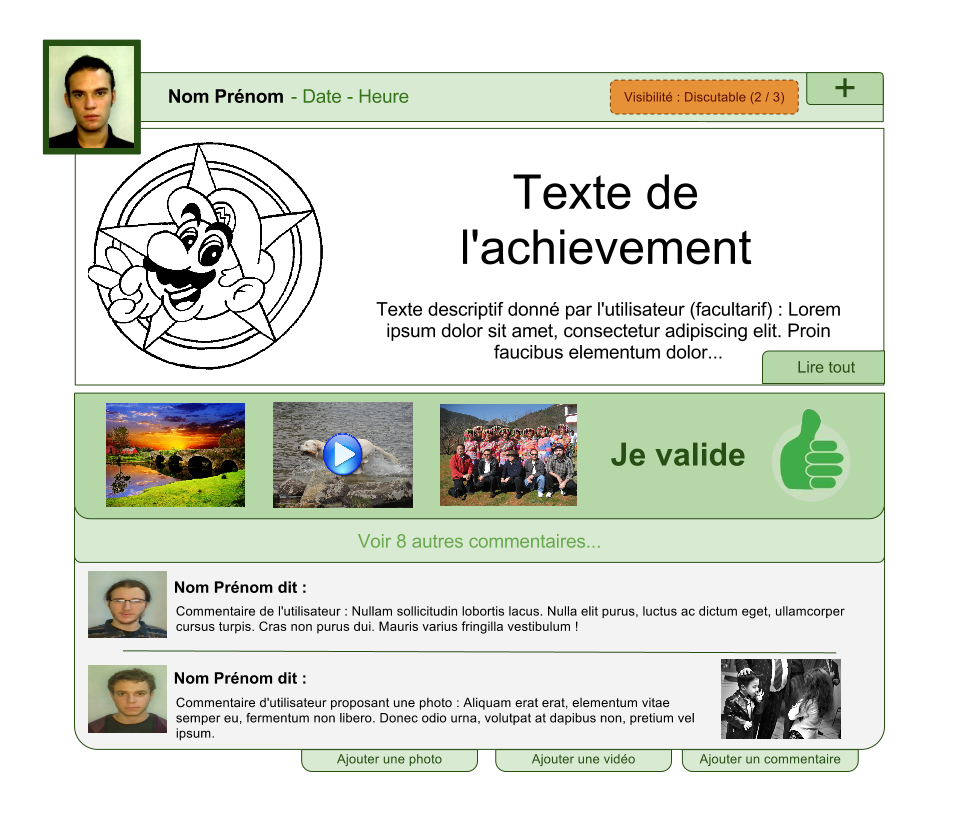
\includegraphics[width=15cm]{img/achievement.png}
  \end{center}
\end{figure}

\subsection{Onglet Achievements}

L'utilisateur pourra sélectionner des packs qui contiendront les achievements à accomplir. Les packs seront tous disponibles et classés par thématiques dans une sous-catégorie, mais la plate-forme proposera d'abord à l'utilisateur des packs d'achievements correspondant aux centres d'intérêt de ce dernier, ou encore de sa tranche d'âge. Une fois un pack sélectionné, l'utilisateur peut aussi définir certains achievements comme étant ses objectifs, et ainsi notifier son réseau.

\subsection{Onglet Objectifs}

L'onglet Objectifs permet à l'utilisateur de construire une “to-do list” ou “bucket-list”, le but étant de filtrer les achievements que l'utilisateur ne désire pas réaliser dans l'immédiat et ainsi de dégager ceux qu'il va accomplir sur le court terme. La page est destinée à être régulièrement consultée : c'est à partir de cet onglet que l'utilisateur peut annoncer la fin d'un objectif, et donc obtenir un achievement si ses amis confirment la validation de ce dernier.

\subsection{Onglet Contacts}

L'utilisateur pourra ici voir sa liste de contacts et les profils de ceux-ci, mais aussi regrouper ses contacts par groupe. Les groupes d'utilisateurs permettent alors d'attribuer des degrés de sensibilité.
Le degré de sensibilité va de 0 à 3 et permet de partager les achievements aux contacts de son choix.

\subsection{Page Profil}
La page Profil contient les informations d'un utilisateur, et permet de les modifier. Si l'utilisateur consulte la page profil d'un autre membre, il a la possibilité d'interagir avec lui de différentes manières (Envoi de message, Demande d'ajout en amis, ...).
La page profil contient principalement des badges d'achievement, tel un tableau de chasse. L'utilisateur peut cliquer sur l'achievement pour en avoir le détails (textes, photos, vidéos, commentaires).

\section{L'application Smartphone}
Pour ce qui est des smartphones, nous avons décidés de ne pas coder dans les langages propres à chaque plates-formes, mais de développer une interface sur la base de la technologie que nous utilisons pour notre site web, à savoir Ocsigen. Cela nous permettra d'être constant dans notre ligne directrice de code. Cette interface sera chargée sur toutes les plates-formes smartphones sous forme d'une web-view. L'avantage de cette méthode réside dans sa totale portabilité qui nous évite d'avoir à développer une application spécifique à chaque plate-forme existante.

\section{L'API}

L'API permettrait d'offrir aux développeurs un accès à l'essentiel des fonctionnalités du site. On pourra y récupérer, pour un utilisateur donné, et selon les vœux de celui-ci (token d'acceptation), la liste de ses achievements.

\chapter{Etude des ressources}

\section{Coûts}

\begin{itemize}
  \item Un compte développeur pour chaque boutique d'application (iOS : AppStore (99\$), Google Play (Android : 25\$) et Marketplace Windows Phone (99\$)) pour les applications mobiles.
  \item Un serveur dédié, dans un premier temps taillé pour le développement du site pouvant gérer seulement peu d'utilisateurs connectés en même temps à environ 15 euros par mois
  \item Un serveur de production, qui sera utilisé ultérieurement pouvant aller jusqu'à 600 euros par mois.
  \item Nous envisageons par la suite, une fois l'application complétement terminée, d'engager un graphiste pour les achievements.
\end{itemize}

\section{Planning}

D'un point de vue global, le projet se déroulera en trois grandes parties : documentation, développement et mise en production.\\

Avant de passer à la réalisation concrète du produit, nous allons nous consacrer à la rédaction de plusieurs documents essentiels au bon déroulement du projet. En effet, il est nécessaire de définir précisément les détails du projet, étudier les différents outils et technologies à notre disposition et faire des choix, ou encore mettre en place des partenariats. Nous continuerons cette étude jusqu'à Septembre 2012.\\

Une fois les outils en main, les spécificités définies et les rôles attribués, nous commencerons à développer le produit. Nous pensons mettre en ligne une version bêta pour Septembre 2013.\\

La dernière période sera consacrée aux problématiques de communication, et dans une moindre mesure de développement. Ainsi, durant la dernière année du projet, nous tâcherons de faire connaître ce dernier de diverses façons, pour créer la communauté indispensable à notre plate-forme, en plus de la finalisation technique du produit. Nous pourrons de ce fait bénéficier de retours utilisateur, afin de corriger les anomalies et peaufiner la plate-forme.

\section{Équipe}

Durant la période de développement du produit, l'équipe dispersée dans plusieurs pays, rendant tout travail en équipe difficile. Nous allons nous répartir les tâches de manière à pouvoir travailler de façon relativement autonome : notre projet étant composé de plusieurs éléments distinct, nous nous arrangerons pour ne pas en partager un entre des membres situés dans les lieux différents.\\

Au niveau de la répartition des rôles: Guillaume Caradec s'occupe de la gestion de projet, et Barbara Lepage dirige la partie technique. Nous sommes bien évidemment tous à la charge du développement et de la rédaction de la documentation.\\

Nous avons à notre disposition divers outils pour nous organiser et communiquer plus facilement :\\

\begin{itemize}
  \item Une mailing-list et un canal IRC, permettant de traiter ensemble de diverses problématiques
  \item Un dossier Google Docs, pour pouvoir partager les documents liés au projet et leur rédaction.
  \item Gtalk, une application de google permettant d'organiser des visio-conférences via navigateur.
  \item Un dépôt Git
  \item L'utilisation de Doodle, pour planifier plus facilement les réunions
\end{itemize}

Les membres du groupe se réuniront toutes les semaines pour parler de l'avancement du projet, des imprévus rencontrés et des objectifs à court terme.

\end{document}
